\documentclass[DIV=12]{scrartcl}
\usepackage{dsfont}
\usepackage{tikz}
\usepackage{caption}
\usetikzlibrary{tikzmark}
\usepackage{amsmath}
\usepackage{amsthm}
\usepackage{amssymb}
\usepackage{amsfonts}
\usepackage{bbm}
\newtheorem{proposition}{Proposition}
\usepackage{graphicx}
\usepackage{hyperref}
\graphicspath{{img/}}
\usepackage[ngerman]{babel}
\usepackage[T1]{fontenc}
\usepackage{comfortaa}
\renewcommand{\sfdefault}{comfortaa}
\title{Einführung in die Theoretische Informatik}
\author{Felix Ichters\thanks{Universität Heidelberg}}
\date{Sommersemester 2023}

\begin{document}
\maketitle
\rule{\textwidth}{0.4pt}
\begin{abstract}
\begin{flushright}
    \textit{Begleitmaterial zur Vorlesung 'Einführung in die Theoretische Informatik'.}
\end{flushright}    
\end{abstract}
\par\bigskip
\begin{center}
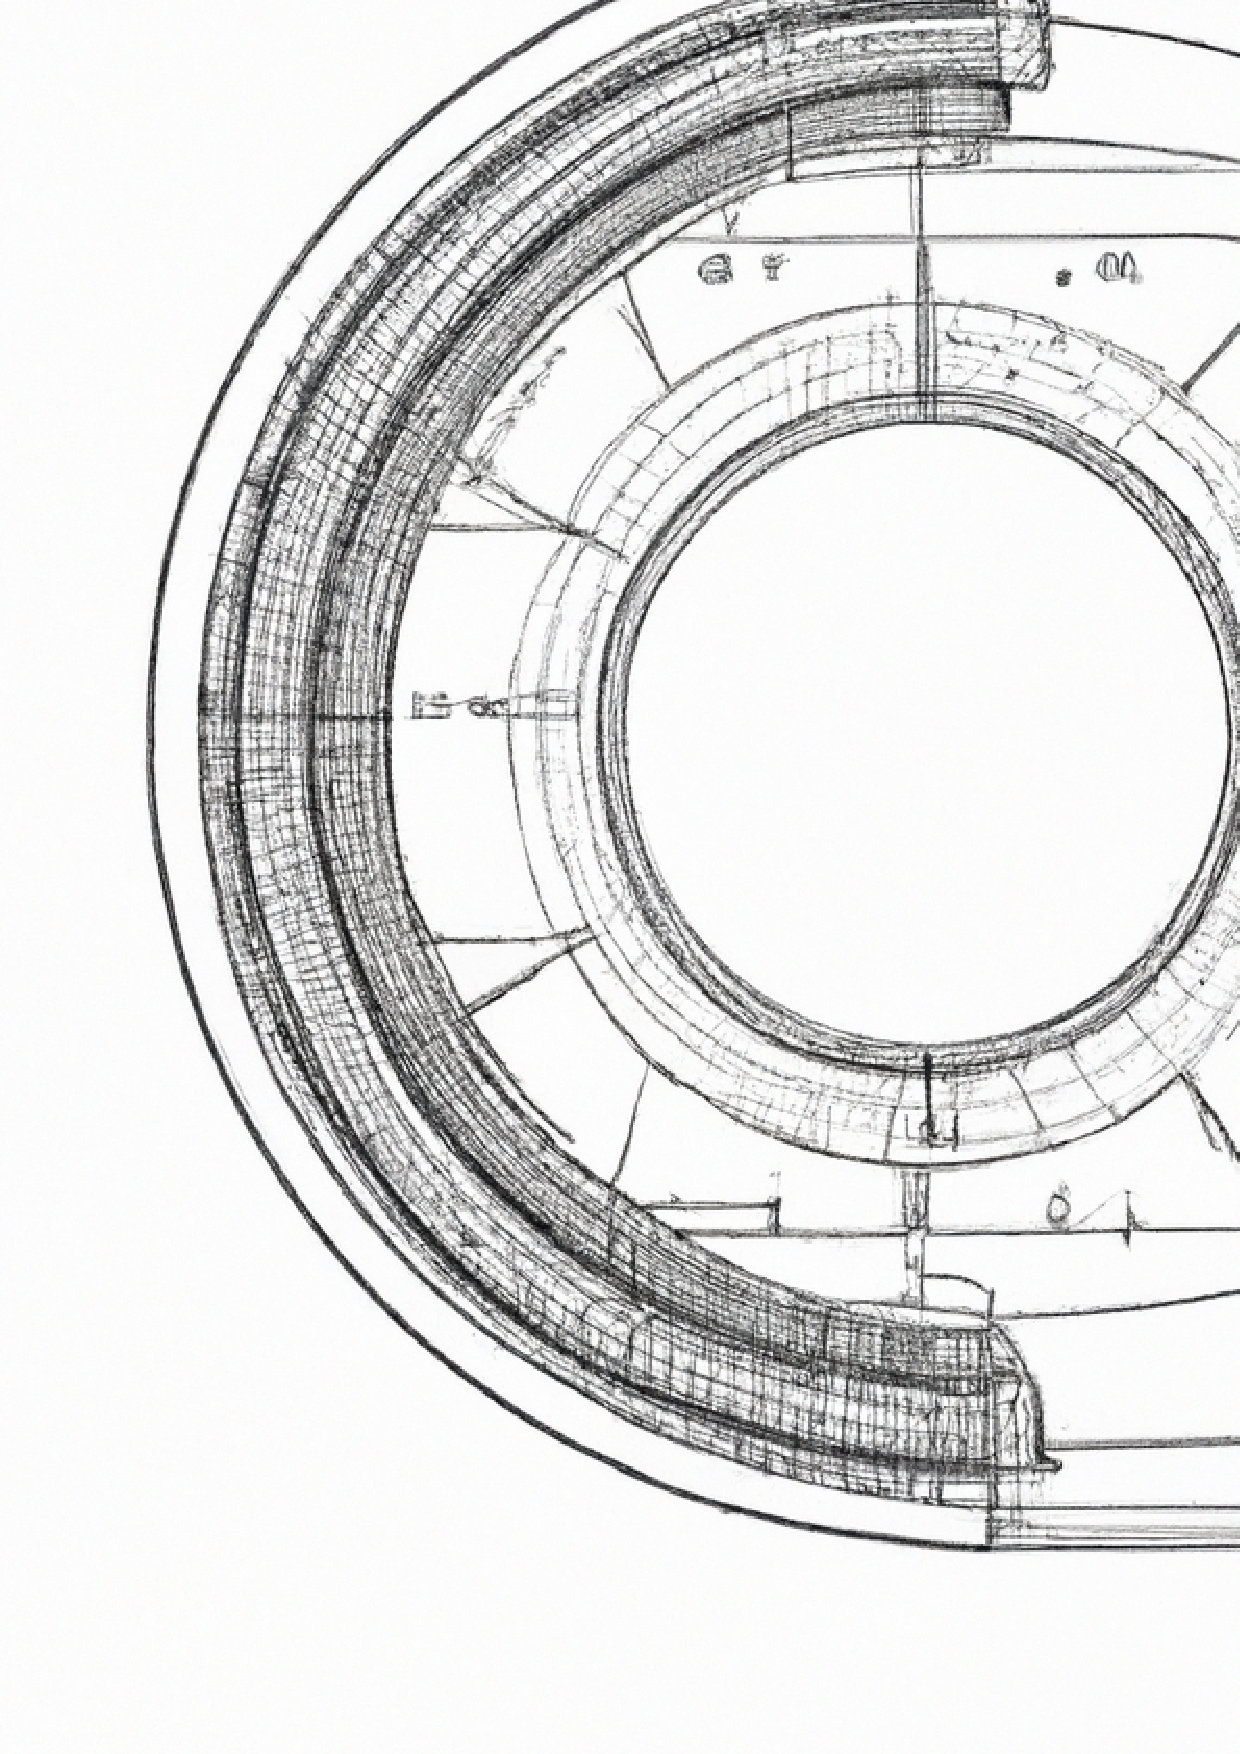
\includegraphics[width=0.5\textwidth]{dall2.png}    
\end{center}

\newpage
\tableofcontents
\newpage
\section*{Notationen}
\begin{itemize}
    \item Für \(n\in\mathbb{N}_0\), sei \([n]=\{1,\dots,n\}\) und \([n]_0=\{0,1,\dots,n\}\).
    \item Für eine Menge A und \(n\in\mathbb{N}\) ist \(A^n=\{(a_1,\dots,a_n):a_1,\dots,a_n\in A\}\).
    \item Für \(n\in\mathbb{N}\) ist eine n-äre partielle Funktion \(\varphi:A^n\rightsquigarrow B\) eine Funktion
    mit \(dom(\varphi)\subseteq A^n\) und \(Im(\varphi)\subseteq B\).
    Für \(a_1,\dots,a_n\in A\) bedeutet \(\varphi(a_1,\dots,a_n)\downarrow\), dass \(a_1,\dots,a_n\in dom(\varphi)\) gilt und 
    \(\varphi(a_1,\dots,a_n)\uparrow\) beduetet, dass \((a_1,\dots,a_n)\notin dom(\varphi)\).
    Die partielle Funktion \(\varphi\) ist total, wenn \(dom(\varphi)=A^n\) gilt.
    \item Eine lineare Ordnung auch totale Ordnung, auf einer Menge A ist eine Relation \(\leq\subseteq A^2\), so dass 
    die folgenden Eigenschaften erfüllt sind
        \subitem \(a\leq a\) \(\forall a\in A\) (Reflexivität)
        \subitem \(a\leq b\wedge b\leq a\Rightarrow a=b\) \(\forall a,b\in A\) (Antisymmetrie)
        \subitem \(a\leq b,b\leq c\Rightarrow a\leq c\) \(\forall a,b,c\in A\) (Transitivität)
        \subitem \(a\leq b\vee b\leq a\) \(\forall a,b\in A\) (Totalität)
\end{itemize}
\section{Grundlagen}
\rule{\textwidth}{0.4pt}
\newpage
\subsection{Alphabet}
    Ein Alphabet ist eine nichtleere Menge \(\Sigma\),die Elemente heißen Symbole.
\subsection{Wörter}
    Ein Wort über einem Alphabet \(\Sigma\) ist eine endliche Folge von Symbolen aus \(\Sigma\).\\
    Für \(i\in[|w|]\) bezeichnet \(w(i)\) das i-te Element von w und für Symbole \(a_1,\dots,a_n\in \Sigma\)
    bezeichnet \(a_1,a_2,\dots,a_n\) das Wort w der Länge n mit \(w(i)=a_i\) \(\forall i\in [n]\).
\subsection{Sprache}
    Eine Sprache ist eine Menge von Wörtern über einem gemeinsamen Alphabet \(\Sigma\).
\subsection{\(\Sigma^*\)}
    Die Menge aller Wörter über \(\Sigma\) wird mit \(\Sigma^*\) bezeichnet.\\
    Für \(n\in\mathbb{N}_0\) setzen wir
    \[\Sigma^{\leq n}:=\{w\in\Sigma^*:|w|\leq n\}\]
    \[\Sigma^{=n}:=\{w\in\Sigma^*:|w|=n\}\]
    \[\Sigma^{\geq n}:=\{w\in\Sigma^*:|w|\geq n\}\]
    \[\Sigma^{+}:=\Sigma^{\geq 1}\]
\subsection{Verkettung}
    Für Wörter \(w_1,w_2\) ist die Verkettung \(w_1w_2\) ist definiert durch 
    \[w_1w_2:=w_1(1)\dots w_1(|w_1|)w_2(1)\dots w_2(|w_2|).\]
    Für Sprachen \(L_1,L_2\) sei \(L_1L_2\) definiert durch 
    \[L_1L_2:=\{w_1w_2:w_1\in L_1, w_2\in L_2\}\]
\subsection{Präfix, Infix, Suffix}
    Seien u,v Wörter 
    \begin{itemize}
        \item u ist Präfix von v, kurz \(u\sqsubseteq v\), falls es ein Wort w gibt, sodass uw=v 
        \item u ist Infix von v, falls es Wörter \(w_1,w_2\) gibt, sodass \(v=w_1uw_2\)
        \item u ist Suffix von v, falls es ein Wort w gibt, sodass v=wu
    \end{itemize}
\subsection{Homomorphismus}
    Für Sprachen \(L,M\) heißt eine Funktion \(\varphi:L\to M\) 
    Homomorphismus von Sprachen, wenn gilt: \[\varphi(uv) = \varphi(u)\varphi(v)\]
\subsection{Längenlexikographische Ordnungen}
    Es gilt \(u \leq_{llex} v\) wenn eine der folgenden Bedingungen erfüllt ist:
    \begin{enumerate}
        \item \(|u|<|v|\)
        \item \(|u|=|v|\) und ist \(i\in[|u|]\) minimal mit \(u(i)\ne v(i)\), so gilt \(u(i)\leq v(i)\)
    \end{enumerate}
\subsection{bin(i)}
\(bin(i)\) ist die Funktion für das in Längenlexikopraphischer Reihnfolge \(i+1\)-te Binärwort.\\
\(1bin(i)\) beschreibt die Binärdarstellung von \(i+1\).
\include{turingmaschienen/turingmaschienen}
\section{Automaten}
\rule{\textwidth}{0.4pt}
\newpage
\subsection{Endlicher Automat}
    Ein endlicher Automat, EA, ist ein Tupel \(A=(Q,\Sigma,\Delta,s,F)\).
    \begin{itemize}
        \item Q ist eine endliche Menge, die Zustandsmenge 
        \item \(\Sigma\) das Eingabealphabet
        \item \(\Delta\subseteq Q\times\Sigma\times Q \) die Übergangsrelation, so dass es 
        für alle \(q\in Q\) und \(a\in\Sigma\) ein \(q'\in Q\) mit \((q,a,q')\)
        \item \(s\in Q\) der Startzustand 
        \item \(F\subseteq Q\) die Menge der akzeptierenden Zustände
    \end{itemize}
    \textit{Der endliche Automat A ist ein deterministischer endlicher Automat, kurz DEA, wenn es
    \(\forall(q,a)\in Q\times\Sigma\) genau ein q' gibt mit \((q,a,q')\in\Delta\).
    Im Sinne der obigen Betrachtung entspricht ein EA \(A=(Q,\Sigma,\Delta,s,F)\) der 1-TM
    \(M_A=(Q,\Sigma,\Sigma\cup\{\square\},\{(q,a,q',a,R):(q,a,q')\in\Delta\},s,F)\).} 
\subsection{Übergangsfunktion eines EA}
    Die Übergangsfunktion eines EA A ist die Funktion \(\delta _A^*(q,\lambda)=\{q\}\) und
    \[\delta_A^*(q,aw)=\bigcup\limits_{q'\in\delta_A(q,a)}\delta_A^*(q',w)\] 
    \(\forall q\in Q,a\in\Sigma, w\in\Sigma^*\)\\
    Für \(Q_0\subseteq Q\) und \(w\in\Sigma^*\) schreiben wir \(\delta_A^*(Q_0,w)\) statt 
    \(\bigcup\limits_{q\in Q_0}\delta_A^*(q,w)\).\par\bigskip
    \textit{Sei A = (Q, $\Sigma$, $\Delta$, s, F) ein EA
    \begin{itemize}
        \item [(i)] $\forall$ q $\in$ Q und a$\in \Sigma$ gilt $\delta_{A}^{*}$(q,a) = $\delta_{A}$(q, a).
        \item [(ii)] Ist A ein DEA, q $\in$ Q, a $\in \Sigma$ und w $\in \Sigma^{*}$, und $\lvert \delta_{A}^{*}(q,w) \rvert$ = 1??.
        \item[(iii)] Seien u,v $\in \Sigma^{*}$ $\forall$ q $\in$ Q gilt $\delta_{A}^{*}$(q, uv) = $\delta_{A}^{*}(\delta_{A}^{*}(Q_{0}, u), v)$.
    \end{itemize}}
\subsection{Übergangsfunktion eines DEA}
    Sei A ein DEA. Auch die Funktion \(\delta_{det,A}:Q\times\Sigma\to Q\) mit \(\delta_a(q,a)=\{\delta_{drt,A}(q,a)\}\)
    \(\forall q\in Q\) und \(a\in \Sigma\) wird Übergangsfunktion von A genannt.
    Analoges gilt für \(\delta_{det,A}^*\) und \(\delta_A^*\).\\
    Für \(Q_0\subseteq Q\) und \(w\in\Sigma^*\) schreiben wir auch \(\delta_{det,A}^*(Q_0,w)\).\par\bigskip
    \textit{Sei Q eine endliche Menge, $\Sigma$ ein Alphabet, s$\in$ Q, und F$\subseteq$ Q. 
    \begin{itemize}
        \item [(i)] $\forall$ Funktionen $\delta$ : Q $\times \Sigma \rightarrow 2^{Q}$ gibt es genau einen EA A = (Q, $\Sigma$, $\Delta$, s, F) mit $\delta_{A}$ = $\delta$.
        \item [(ii)] $\forall$ Funktionen $\delta$ : Q $\times \Sigma \rightarrow$ Q gibt es genau einen $\delta_{det, A}$ = $\delta$. 
    \end{itemize}}
\subsection{akzeptierte Sprache}
    Sei A ein EA. Die Sprache \(L(A):=\{w\in\Sigma^*:\delta_A^*(s,w)\cap F\neq\varnothing\}\) ist die akzeptierte Sprache von A. 
\subsection{Regulär}
    Eine Sprache L heißt regulär, wenn es einen EA A mit L(A)=L gibt.\\
    Wir schreiben REG für die Klasse der regulären Sprachen.
    \subsubsection*{Beispiel}
    \textit{Zu jedem Zeitpunkt während der Verbindung der Eingabe durch einen endlichen Automaten höngt der restliche Bearbeitung immer nur vom gegewärtigen Zustand und dem noch einzulesenden Teil der Eingabe ab, nicht aber wie bei TM im allgemeinen von vergangenen Bandmanipulation. Interpretiert man die Eingabe als von einer äußeren Quelle kommend, so ist der  Zustand des Automaten also allein durch seinen Zustand gegeben und der nächste Zustand hängt nur vom Zugeführten Symbol ab. Daher bietet sich eine Darstellung eines EA durch ein Übergangsdiagramm oder eine sogenannte Übergangstabelle an.}\\
    Sei A := (\{$q_{0}$, $q_{1}$\}, \{0, 1\}, $\Delta$, $q_{0}$, \{$q_{1}$\}) mit $\Delta$ = \{($q_{0}$)\}
Übergangsdiagramm und übergangstabelle von sehen wie folgt aus:
\begin{center}
    \begin{tabular}{|c|c|c|}
        \hline
        Zustand/Symbol & 0 & 1 \\
        \hline
        $q_{0}$ & $q_{0}$ & $q_{1}$ \\
        \hline
        $q_{1}$, * & $q_{1}$ & $q_{0}$ \\
        \hline
    \end{tabular}            
\end{center}
\subsection{Übergangsdiagramm}
    Für jeden Zustand gibt es einen Kreis. Zustände in F bekommen einen Doppelkreis. Für \((q,a,q')\in\Delta\) für wir 
    einen Pfeil von dem Kreis von q zu dem Kreis von q' mit der Beschriftung a.\\
    Zustätzlich gibt es einen Pfeil (ohne Beschriftung) aus dem 'Nichts' zu dem Kreis des Startzustandes.
\subsection{Potenzautomat}
    Sei A ein EA. Der Potenzautomat von A ist der DEA \(P_a=(2^Q, \Sigma, \Delta',\{s\},\{P\subseteq Q:P\cap F\neq\varnothing\})\) mit
    \[\delta_{det,P_a}(Q_0,a)=\bigcup\limits_{q\in Q_0}\delta_A(q,a)\text{ }\forall Q_0\subseteq Q\text{ }\forall a\in\Sigma\]
    \subsubsection*{Satz}
        Eine Sprache L ist genau dann regulär, wenn es einen DEA A mit L(A) = L gibt.\par\bigskip
        \begin{proof}
            Sei A = (Q, $\Sigma$, $\Delta$, s, F) ein EA mit Potenzautomat $P_{A}$. Es genügt zu zeigen, dass L(A) = L($P_{A}$). Hierfür genügt es zu zeigen, dass:
\[\delta_{det,P}^{*} = \delta_{A}^{*}(s, w) \forall w \in \Sigma^{*} (*)\]
Denn damit folgt
\[w \in  L (P_{A}) \Leftrightarrow \delta_{P_{A}}^{*}(\{s\}, w) \cap \{P\subseteq Q : P\cap F \neq \varnothing \} \neq \varnothing \] 
\[\Leftrightarrow \delta_{det, P_{A}}^{*}(\{s\}, w) \cap F \neq \varnothing \]
\[\underset{\text{(*)}}{\Leftrightarrow } \delta_{A}^{*}(\{s\}, w) \cap F \neq \varnothing \]
\[\Leftrightarrow w \in L(A)\] Wir zeigen (*) mittels vollständiger Induktion über $\lvert$w$\rvert$. Es gilt $\delta_{det, P_{A}}^{*}$(\{s\}, $\lambda$) = $\delta_{A}^{*}$(s, $\lambda$). Sei w $\in \Sigma^{+}$ mit $\delta_{det, A}^{*}$(\{s\}, v) = $\delta_{A}^{*}$(s, v) $\forall$ v $\in \Sigma^{\leq \lvert w \rvert - 1}$. Nun zeigen wir (*) Sei va := w mit a $\in \Sigma$ und $\lvert$v$\rvert$ = $\lvert$w$\rvert$ - 1.
\[\delta_{det, P_{A}}^{*} (\{s\}, w) \underset{\text{Bem 4.5}}{=} \delta_{det, P_{A}}^{*} (\delta_{det, P_{A}}^{*}(\{s\}, v), a)\]
\[\underset{\text{Ind. hyp}}{=} \delta_{det, P_{A}}^{*}(\delta_{det, P_{A}}^{*}(\{s\}, v), a)\]
\[ = \bigcup \limits_{q \in \delta_{det, A}^{*}}\delta_{A}(q, a)\]
\[ = \delta_{A}^{*}(\delta_{A}^{*}(s, v), a)\]
\[ = \delta_{A}^{*}(s, va)\]
\[ = \delta_{A}^{*}(s, w)\]
        \end{proof}
\section{Reguläre Sprachen}
\rule{\textwidth}{0.4pt}
\textit{Wir verschieben den Fokus von endlichen Automaten auf die Klasse der von diesen erkannten Sprachen.
Dabei spielen endl. Automaten weiterhin eine wichtige Rolle.
Wegen 4.7 beschränken wir uns auf deterministische endliche Automaten.\\
Sei A DEA. Die Menge der zulässigen Eingaben \(\Sigma^*\) ist unendlich groß, 
die Menge der Zustände Q is aber endlich. Zwangsläufig wir A also das Einlesen verschiedener 
Eingaben im gleichen Zustand abschließen (und somit gleich behandeln). Dies führt zum Begriff
der A-Äquivalenz.}
\subsection{Äquivalenzrelation}
    Sei A eine Menge. Eine Äquivalenzrelation auf A ist eine Relation \(\sim\subseteq A²\), so dass
    die folgenden Eigenschaften erfüllt sind.
    \begin{enumerate}
        \item \(a\sim a\) \(\forall a\in A\) (Reflexivität)
        \item \(a\sim b\Rightarrow b\sim a\) \(\forall a,b \in A\) (Symmetrie)
        \item \(a\sim b, b\sim c\Rightarrow a\sim c\) \(\forall a,b,c\in A\) (Transitivität)
    \end{enumerate}
    Die Äquivalenzklasse eines Elements \(a\in A\) bezüglich \(\sim\) ist die Menge 
    \([a]_\sim:=\{a'\in A:a'\sim a\}\). Der Index von \(\sim\) isr die Kardinalität
    der Menge \(A/{\sim}:=\{[a]_\sim:a\in A\}\) falls diese endlich ist und unendlich andernfalls.
\subsection{A-Äquivalenz}
    Sei A ein DEA. mit erweiterter Übergangsfunktion \(\delta^*:Q\times\Sigma\to Q\).\\
    Die A-Äquivalenz ist die Relation \(\sim_A\) auf \(\Sigma^*\) mit 
    \[u\sim_A v\Leftrightarrow \delta^*(s,u)=\delta^*(s,v)\text{ }\forall u,v\in\Sigma^*\]\par\bigskip
    \textit{\begin{itemize}
        \item [(i)] Die A-Äquivalenz ist eine Äquivalenzrelation.
        \item [(ii)] Der Index von $\sim_{A}$ ist höchstens $|Q|$.
        \item [(iii)] Es gilt $L(A) = \bigcup \limits_{w \in L(A)} [w]_{\sim A}$.
    \end{itemize}}
\subsection{Rechtskongurenz}
    Sei \(\Sigma\) ein Alphabet. Eine Rechtskongurenz auf \(\Sigma^*\) ist eine Äquivalenzrelation
    \(\sim\subseteq(\Sigma^*)^2\) mit \\
    \(u\sim v\Rightarrow uw\sim vw\) \(\forall u,v,w\in\Sigma^*\).
    \subsubsection*{Proposition}
    Sei $A = (Q, \Sigma, \Delta, s, F)$ ein DEA. Die A-Äquivalenz $\sim_{A}$ ist eine Rechtskonqruenz auf $\Sigma^{*}$.
        \begin{proof}
          Seien $u, v, w \in \Sigma^{*}$ mit $u \sim_{A} v$. Dann gilt 
          \[\delta_{det, A}^{*}(s, uw) = \delta_{det,A}^{*}(\delta_{det,A}^{*}(s, u), w) = \delta_{det,A}^{*}(\delta_{det,A}^{*}(s,v), w)\]
          \[= \delta_{det,A}^{*}(s, vw).\]
          Dann gilt $uw\sim_{A}vw.$    
        \end{proof} 
        Zu jedem DEA A gibt es also eine dazugehärige Rechtskonguenz $\sim$ auf $\Sigma^{*}$ mit endlichem Index so dass L(A) die Vereinigung von Äquivalenzklasse von $\sim_{A}$ ist. Tatsächlich gilt auch die Umkehrung: Ist L die Vereinigung von Äquivalenzklasse einer Rechtskongruenz $\sim$ mit endlichem Index, so gibt es einen DEA A mit $L(A) = L$.
\subsection{}
    Sei \(\Sigma\) ein Alphabet und L Vereinigung von Äquivalenzklassen einer Rechtskongurenz \(\sim\)
    auf \(\Sigma^*\) mit endlichem Index. Es bezeichne 
    \[A_{\sim,L}:=(\Sigma^*/{\sim},\Sigma,\Delta,[\lambda]_\sim,\{[w]_\sim:w\in L\})\]
    den DEA mit \(\delta_{det,A_{\sim,L}}([w]_\sim,a)=[wa]_\sim\) \(\forall w\in\Sigma^*\) und \(a\in\Sigma\).
    \subsubsection*{Lemma}
    Sei $\Sigma$ ein Alphabet, L Vereinigung von Äquivalenzklassem einer Rechtskongruenz $\sim$ auf $\Sigma^{*}$ mit endlichem Index und sei $\delta^{*} : \Sigma^{*}_{/\sim} \times \Sigma^{*} \rightarrow \Sigma^{*}_{/\sim}$ die erweiterte Übergangsfunktion von $A_{\sim, L}$. Dann gilt $\delta^{*}([\lambda]_{\sim}, w) = [w]_{\sim} \forall w \in \Sigma^{*}$. 
\begin{proof}
  Wir verwenden vollständige Induktion über $|w|$. Es gilt $\delta^{*}([\lambda]_{\sim}, \lambda) = [\lambda_{\sim}]$. Sei nun $w \in \Sigma^{+}$ mit \(\delta^*([\lambda]_\sim,v)\) \(\forall v\in\Sigma^{\leq|w|-1}\). Es genügt zu zeigen, dass \(\delta^*([\lambda]_\sim,w=[w]_\sim)\).\\
  Sei \(va=w\) mit \(a\in\Sigma\)\\
  Dann gilt \(\delta^*([\lambda]_\sim,w)=\delta^*(\delta^*([\lambda]_\sim,v),a)=\lambda^*([v]_\sim,a)=[va]_\sim=[w]_\sim\)
\end{proof}
\subsubsection*{Satz} Sei L die vereinigung von Äquivalenzklasse einer Rechtskongruenz $\sim$ mit endlichem Index Es gibt $L(A_{\sim, L}) = L$ 
\begin{proof}
  Sei $\Sigma$ das Alphabet, so dass $\sim$ eine Rechtskongruenz auf $\Sigma^{*}$ ist. Sei $\delta^{*} : \Sigma^{*}_{/\sim} \times \Sigma^{*} \rightarrow \Sigma^{*}_{/\sim}$ die erweiterte Übergangsfunktion von $A_{\sim, L}$ und sei $w \in \Sigma^{*}$. Es folgt 
  \[w \in L(A_{\sim, L}) \Leftrightarrow \delta^{*}([\lambda]_{\sim}, w) \in {[v]_{\sim} : v \in L}\]
  \[\Leftrightarrow [w]_{\sim} \in {[v]_{\sim} : v\in L}\]
  \[\Leftrightarrow \exists v \in L : [w]_{\sim} = [v]_{\sim}\]
  \[\Leftrightarrow \exists v \in L : w \sim v\]
  \[\Leftrightarrow w \in L\] 
\end{proof}

\subsubsection*{Korollar} Eine Sprache L ist genau dann regulär, wenn sie die Verienigung von Äquivalenzklasse einer Rechtskongruenz mit endlichem Index ist. 
\begin{proof}
  Folgt aus Bemerkung 5.3, Proposition 5.5 und Satz 5.8 $\Box$ 
\end{proof}
Betrachten man nur deterministische endliche Automaten ohne unerreichbare Zustände, so entsprechen diese bis auf Unbenutzung von Zuständen sogar den Rechtskongruenz mit endlichem Index zusammen mit Vereinigung von Äquivalenzklassn dieser.
\subsection{Erreichbar}
    Sei \(\Sigma\) ein Alphabet. Sei A ein EA mit erw. Übergangsfunktion \(\delta^*\). 
    Ein Zustand \(q\in Q\) heißt erreichbar in A wenn es ein Wort \\
    \(w\in\Sigma^*\) mit \(q\in\delta^*(s,w)\) gibt.
\subsection{Isomorph}
    Sei \(A_i\)für \(i\in\{1,2\}\) ein EA mit Übergangsfunktion \(\delta_i\).\\
    Die endlichen Automaten \(A_1\) und \(A_2\) sind Isomorph, kurz \(A\cong A_2 \), wenn es eine Projektion \\ \(f:Q_1\to Q_2\) gibt, so dass folgendes gilt:
    \begin{enumerate}
        \item \(f(s_1)=s_2\)
        \item \(\delta_2(f(q_1),a)=f(\delta_1(q_1,a))\) \(\forall q_1\in Q,a\in\Sigma\)
        \item \(f(F_1)=F_2\)
    \end{enumerate}
    \subsubsection*{Satz}
    \begin{itemize}
        \item [(i)] Ist $A$ ein DEA ohne unereichbare Zustände, so gilt $A \cong A_{\sim A, L(A)}$
        \item [(ii)] Ist L die Vereinuíngung von Äquivalenzklasse einer Rechtskongruenz $\sim$ mit endlichem Index, so gilt $(\sim, L) = (\sim_{A_{\sim, L}, L(A_{\sim, L})})$.
      \end{itemize}
    
      \begin{proof}
        \begin{itemize}
          \item [(i)] Sei $A = (Q, \Sigma, \Delta, s, F)$ eine DEA mit erweiterte Übergangsfunktion $\delta^* : Q \times \Sigma^* \to Q$ ohne unereichbare Zustände , $\sim := \sim_A$, $A' := A_{\sim, L(A)}$ und sei $\delta' : \Sigma^* / \sim \times \Sigma^* \to \Sigma/\sim$ die erweiterte Übergangsfunktion von $A'$. Sei $f : Q \to \Sigma^* / \sim$ die Bijektive mit $f(q) := \{ w \in \Sigma^* : \delta^*(s,w) = q\}$. Es gelte $f(s) = [\lambda]_{\sim}$ und $f(F) = \{[w]_{\sim} : w \in L(A)\}$. Es genügt somit zu zeigen , dass $\delta'(f(q), a) = f(\delta(q,a)) \forall q \in Q, a \in \Sigma$. Sei $q \in Q, a \in \Sigma^*$. Es genügt $w \in \delta' (f(q), a) \Leftrightarrow \delta^*(s,w) = \delta^*(q, a)$ zu zeigen. Sei $v \in \Sigma^*$ mit $\delta^*(s,v) = q$. Nun gilt $w \in \delta'(f(q), a) \leftrightarrow w \in \delta'([v]_{\sim}, a) \leftrightarrow w \sim va \leftrightarrow \delta^*(s,w) = \delta^*(s, va) \leftrightarrow \delta^*(s,w) = \delta^*(q,a)$
          \item [(ii)] Sei $\Sigma$ ein Alphabet, $\sim$ eine Rechtskongruenz aud $\Sigma^*, L$ Vereinigung von Äquivalenzklassen von $\sim$, $A' := A_{\sim, L} = (\Sigma^*/\sim, \Sigma, A', [\lambda]_{\sim}, \uparrow)$, $\delta'^* : \Sigma^*/\sim \times \Sigma^* \to \Sigma^*/\sim$ die erweiterterte Übergangsfunktion von $A'$ $\{w \in \Sigma^* : w \in L \}$ und $\sim' := \sim_{A'}$. Nach Satz 5.8 gilt $L = L(A')$, es genügt also $\sim = \sim'$ zu zeigen. Sei $u, v \in \Sigma^*$. Es folgt $u \sim v \leftrightarrow 
          [u]_{\sim} = [v]_{\sim} \leftrightarrow \delta'([\lambda]_\sim,u)=\delta'([\lambda]_\sim,v)\Leftrightarrow u\sim v$
        \end{itemize}
      \end{proof}
\subsection{L-Äquivalenz}
    Sei L eine Sprache über einem Alphabet \(\Sigma\). Die L-Äquivalenz von L als Sprache ist die Relation \(\sim_L\) auf \(\Sigma^*\) mit 
    \[u\sim_L v\Leftrightarrow(uw\in L\Leftrightarrow vw\in L\text{ }\forall w\in\Sigma^*)\] 
    \subsubsection*{Bemerkung}
        Sei L eine Sprache über \(\Sigma\).
        \begin{enumerate}
            \item Die l-Äquivalenz ist eine Rechtskongurenz
            \item Es gilt \(L=\bigcup_{w\in L}[w]_{\sim L}\)
        \end{enumerate}
\subsection{Partition}
    Sei A eine Menge. Eine Partition von A ist eine Menge \(\mathcal{A}=\{A_1,\dots,A_n\}\) paarweise disjunkte nichtgeliche Teilmengen von A mit \(\bigcup_{i\in[w]}A_i=A\)
\subsection{Verfeinerung}
    Seien \(\mathcal{A}_1\) und \(\mathcal{A}_2\) Partitionen einer Menge A. Die Partition \(\mathcal{A}_2\) verfeinert \(\mathcal{A}_1\), wenn es \(\forall A_2\in\mathcal{A}_2\) ein \(A_i\in\mathcal{A}_1\), mit....
    \textit{
        Seien \(\mathcal{A}_1\) und \(\mathcal{A}_2\) Partitionen eine Menge A, so dass \(\mathcal{A}_2\) die Partition \(\mathcal{A}_1\) verfeinert.
        \begin{enumerate}
            \item \(\forall A'\in\mathcal{A}_1\), gibt es eine Teilmenge \(\mathcal{A}'_2\in\mathcal{A}_2\), die eine Partition von \(A'\) ist
            \item Es gilt \(|\mathcal{A}_1|\leq|\mathcal{A}_2|\)
            \item Gilt \(|\mathcal{A}_1|=|\mathcal{A}_2|\) dann ist \(\mathcal{A}_1=\mathcal{A}_2\)
        \end{enumerate}}
    \subsubsection*{Proposition}
        \textit{Seien \(\Sigma\) ein Alphabet und L eine Sprache über \(\Sigma\) und \(\sim\) eine Rechtskongurenz auf \(\Sigma^*\) mit \(L=\bigcup_{w\in L}[w]_\sim\). Die Partition \(\Sigma^*\backslash\sim\) ist eine Verfeinerung der Partition \(\Sigma^*\backslash\sim_L\).}\par\bigskip
    \begin{proof}
        Seien \(u,v\in\Sigma^*\) mit \(u\sim v\). Es genügt zu zeigen, dass \(u\sim_Lv\).\\
        Sei \(w\in\Sigma*\). Es genügt \(uw\in L\Leftrightarrow vw\in L\) zu zeigen.\\
        Da \(\sim\) eine Rechtskongurenz ist folgt \(uw\sim vw\). Ist \(uw\in L\), so folgt aus \(L=\bigcup_{w'\in L}[w']_\sim\) auch \(vw\in L\) (analog folt auch \(vw\in L\Rightarrow uw\in L\)).\\
        \(\Rightarrow u\sim_Lv\)\\
    \end{proof}
        D.h. \(\sim_L\) ist die gröbste Partition, die L darstellen kann.
\subsection{Minimalautomat}
    Sei L eine reguläre Sprache über \(\Sigma\). Der Minimalautomat von L als Sprache über \(\Sigma\) ist der DEA \(A_{\sim_{L,L}}\)
    \subsubsection*{Satz}
        Sei L eine reguläre Sprache über \(\Sigma\) und sei M der Minimalautomat von L. Dann gilt:
        \begin{enumerate}
            \item[(i)]\(L(M)=L\)
            \item[(iii)]ist A ein DEA mit Zustandsmenge \(Q_A\) und \(L(A)=L\), so gilt \(|Q_A|\geq|Q|\)
            \item[(iii)]ist A ein DEA mit \(|Q|\) Zuständen und \(L(A)=L\), so gitl \(A\cong M\) 
        \end{enumerate}
        %unvolständig-----------------------------------------------
        \begin{proof}
            \begin{enumerate}[label=(\roman*)]
                \item folgt aus vorigem Satz 
                \item Aus voriger Bemerkung folgt \(|Q_A|\geq|\Sigma/_A|\). Nach voriger Proposition ist \(\Sigma^*/_{\sim_A}\) eine Verfeinerung\dots
                \item Sei A ein DEA mit \(|Q|\) Zuständen und \(L(A)=L\).\\
                Hätte A unereichbare Zustände, so folgt \(|\Sigma^*/_{\sim_A}|<|Q|<|\Sigma/_{\sim_L}|\)\dots
            \end{enumerate}
        \end{proof}
        %-----------------------------------------------------------
\subsection{Satz von Myhill und Nerode}
    Für eine Sprache L über einem Alphabet \(\Sigma\) sind die folgenden Aussagen äquivavlent:
    \begin{enumerate}[label=(\roman*)]
        \item L ist regulär 
        \item Der Index von \(\sim_L\) ist endlich
        \item L ist die Vereinigung von Äquivavlenzklassen einer Rechtskongruenz mit endlichem Index 
    \end{enumerate}
    \begin{proof}
        \begin{enumerate}[label=(\roman*)]
            \item \(\Leftrightarrow\) (iii) ist die Aussage von vorigem Korollar\\
            Die Relation \(\sim_L\) ist eine Rechtskongruenz und es gilt \(L=\bigcup_{w\in L}[w]_{sim_L}\). Somit folgt (ii)\(\Rightarrow\) (iii).\\
            Die Implikation (iii) \(\Rightarrow\) (ii) folgt.
        \end{enumerate}
\subsection{Pumping-Lemma}
    \textit{Wir wollen nun ein Kriterium beschreiben das hilft nicht reguläre Sprachen zu erkennen}\par\bigskip
    Sei \(\Sigma\) ein Alphabet. Für jede reguläre Sprache \(L\subseteq\Sigma^*\) gibt es eine Konstante \(k\in\mathbb{N}\), so dass folgendes gilt:\\
    Ist \(z\in L\) mit \(|z|\geq k\), so gibt es Wörter \(u,v,w\in\Sigma^*\) mit \(z=uvw\), so dass folgendes gilt:
    \begin{enumerate}[label=(\roman*)]
        \item \(v\not=\lambda\)
        \item \(|uv|\leq k\)
        \item \(uv^iw\in L\) \(\forall i\in\mathbb{N}_0\)
    \end{enumerate} 
    \end{proof}
    \paragraph*{Beweis}
        Sei \(L\subseteq\Sigma^*\) eine reguläre Sprache und A ein DEA mit L(A)=L und erweitereter Übergangsfunktion \(\delta^*:Q\times\Sigma^*\to Q\).\\
        Sei \(k:=|Q|\).\\
        Sei \(z\in L\) mit \(|z|\geq k\). (Falls kein solches z existiert ist nichts zu zeigen)\\
        Die Funktion \(f:\{0,\dots,k\}\to Q\), \(i\to \delta^*(s,z(1),\dots,z(i))\) ist keine Injektion, denn es gilt \(|\{0,\dots,k\}|=k+1>|Q|\). Seien \(j_1,j_2\in\{0,\dots,k\}\) mit \(j_1<j_2\) und \(f(j_1)=f(j_2)\).\\
        Sei \(u:=z(1)\dots z(j_1),v=z(j_1+1)\dots z(j_2),w=z(j_2+1)\dots z(|z|)\).\\
        Dann gilt \(z=uvw\).\\
        Aus \(j_1<j_2\) folgt \(v\not=\lambda\).\\
        Aus \(j_2\leq k\) folgt \(|uv|\leq k\).\\
        Es bleibt zu zeigen, dass \(uv^iw\in L\) \(\forall i\in\mathbb{N}_0\) gilt.\\
        Dafür genügt es zu zeigen \(\delta^*(s,uv^i)=\delta^*(s,u)\).\\
        Denn dann gilt\\
        \[\delta^*(s,uv^iw)=\delta^*(\delta^*(s,uv^i),w)=\delta^*(\delta^*(s,u),w)=\delta^*(\delta^*(s,uv)w)=\delta^*(s,uvw)\] und damit \(uv^iw\in L\).\\
        Wir zeigen \(\delta^*(s,uv^i)=\delta^*(s,u)\) mittels vollständiger Induktion über i.\par\bigskip 
        i=0\\
        Gelte nun \(\delta^*(s,uv^{i-1})=\delta^*(s,u)\) für ein \(i\in\mathbb{N}\)\\
        Wieder folgt \[\delta^*(s,uv^i)=\delta^*(\delta^*(s,uv^{i-1}),v)=\delta^*(\delta^*(s,u),v)=\delta^*(s,uv)=f(j_2)=f(j_1)=\delta^*(s,u)\]
    \paragraph*{Beispiel}
    Die Sprache \(L=\{0^n1^n:U\in\mathbb{N}_0\}\) ist nicht regulär Dies lässt sich mit dem Pumping-Lemma wie folgt zeigen.
    \begin{proof}
        \(\Rightarrow\exists k\in\mathbb{N}_0:\forall z\in L\) mit \(|z|\geq k\) gilt, \(\exists u,v,w\in\Sigma^*\) mit \(z=uvw\) und (i)(ii)(iii) aus Pumping.\\
        Sei \(z:=0^k1^k\).\\
        Aus (i) und (ii) folgt, dass \(v=0^l\) für \(l>0\) und damit folgt\\
        \(uw=0^{k-l}1^k\in L\) nach Pumping-Lemma. Dies ist ein Widerspruch das \(L=\{0^n1^n:u\in\mathbb{N}_0\}\)
    \end{proof}
\end{document}